% -*- TeX-master: "paper.tex"; TeX-PDF-mode: t; ispell-local-pdict: "words" -*-



\section{Design and Implementation}
\label{sec:design}

In this section, we provide details of the design and implementation
of \DeDe's best-effort write
monitoring subsystem and the out-of-band indexing and duplicate
elimination process.

\subsection{Write Monitoring}
\label{sec:idea:stale-wlog}

%%%%%%%%%%%%%%%%%%%%%%%
%%%% Figure %%%%%%%%%%%
%%%%%%%%%%%%%%%%%%%%%%%

\begin{figure}[t]
\centerline {
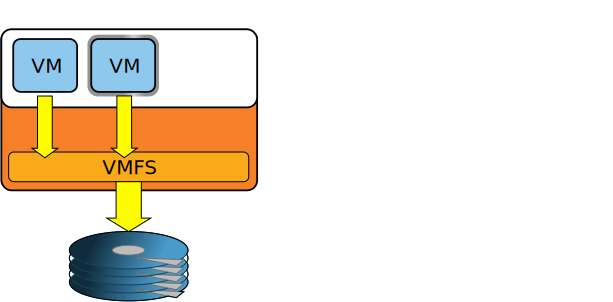
\includegraphics[scale=0.45]{figures/writemon.pdf}
}
%\vspace{-0.2in}
\caption{Only a lightweight kernel module lies
  in the IO critical path, opportunistically calculating hashes of
  blocks while they are still in memory. A userspace daemon ({\tt
    \small dedupd}) flushes write logs to disk periodically. Duplicate
  detection and elimination occur out of band.}
%\vspace{-0.1in}
\label{fig:write-monitoring}
\end{figure}

%%%%%%%%%%%%%%%%%%%%%%%
%%%% /Figure %%%%%%%%%%
%%%%%%%%%%%%%%%%%%%%%%%

Each host runs a \emph{write monitor}, as shown in
Figure~\ref{fig:write-monitoring}, which consists of a lightweight
kernel module ({\tt \small dedup}) that monitors all writes by that host
to files in the file system and a userspace daemon ({\tt \small dedupd}) that
records this information to logs stored in the shared file system.
The write monitor is the only part of the system that lies in the
IO critical path of the file system, so the write monitor itself must
incur as little additional disk IO and CPU overhead as possible.

% We divide deduplication into separate monitoring and merging processes
% in order to minimize the impact of the system on regular file system
% reads and writes, so we must ensure that the write monitor itself
% incurs as little additional disk IO and CPU overhead as possible.

The kernel module provides the userspace daemon with a modification
stream indicating, for each write done by the host: the file modified,
the offset of the write, and the \shaone hashes of all modified
blocks.  While the in-band CPU overhead of the monitor could have been
virtually eliminated by computing these hashes lazily (\eg, at
indexing time), this would have required reading the modified blocks
back from disk, resulting in a large amount of additional random IO.
We opted instead to eliminate the extra IO by computing these hashes
while the blocks were in memory, though the trade-off between run-time
CPU overhead and deduplication-time IO overhead could be set
dynamically by user-defined policy.

The userspace daemon divides the modification stream by file,
aggregates repeated writes to the same block, and buffers this
information in memory, periodically flushing it to individual write
log files associated with each regular file.  These write logs are
stored on the shared file system itself, so even if
a host fails or transfers ownership of a file's lock, any other host
in the system is capable of reading logs produced by that host and
merging information about modified blocks into the index.

The daemon can safely buffer the modification stream in memory because
the index update process is designed to deal with stale
information.  Without this, write logs would have to be consistent
with on-disk file state, and each logical write to the file system
would result in at least
two writes to the disk.  Instead, buffering allows our system to
absorb writes to over 150~MB of file blocks into a single infrequent
1~MB sequential write to a log file.  This is the only additional IO
introduced by the write monitor.
% (/ (/ (* (/ (* 1024 1024) (+ 20 4)) 4096) 1024) 1024)
% XXX One word overflow, but prevents orphan

Similarly, we rely on the best-effort property of write monitoring to
minimize IO in the case of partial block writes.  If a write
to the file system does not cover an entire block, the monitor simply
ignores that write, rather than reading the remainder of the block
from disk simply to compute its hash.  In practice, this is rarely a
problem when writes originate from a virtual machine, because guest
operating systems typically write whole guest file system blocks,
which are generally at least 4~KB.\footnote{Unfortunately, owing to an
  ancient design flaw in IBM PC partition tables, guest writes are not
  necessarily \emph{aligned} with \DeDe blocks.
  Section~\ref{sec:vmware-vdi-analysis} has a more detailed
  analysis of this.}
% USENIX technically forbids footnotes, but this doesn't make sense as
% an endnote and I've seen USENIX papers use footnotes before.

Write monitoring can be enabled or disabled per file.
If the performance of some VM is too critical to incur the
overhead of write monitoring or if the system administrator has
a priori knowledge that a VM's duplication ratio is small, such VMs
can be opted out of deduplication.

\subsection{The Index}

%%%%%%%%%%%%%%%%%%%%%%%
%%%% Figure %%%%%%%%%%%
%%%%%%%%%%%%%%%%%%%%%%%

% \begin{figure*}
% \centerline {
% 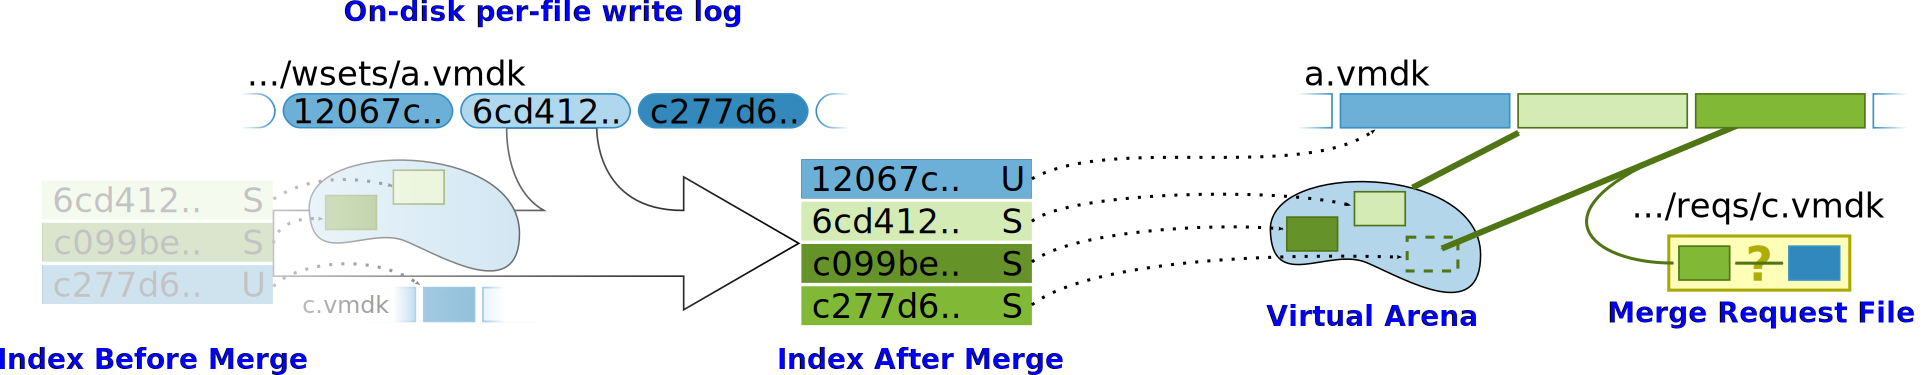
\includegraphics[width=6.0in]{figures/indexing-merging.pdf}
% }
% %\vspace{-0.2in}
% \caption{Indexing and Merging: The index is a map from hash to
%   offsets. For shared blocks (S), the offset is in the virtual arena
%   file whereas for unique blocks (U), it is in a reguar file. Hosts
%   process write logs for their files against the index and zip the two
%   together. The left side of the figure is before a merge operation
%   and the right is after. The entry in the index for c277d6... was
%   converted from a hint unique entry (U) to a shared one (S). As part
%   of that, the host performing that operation left a merge request
%   for whichever host owned file c.vmdk.}
% %\vspace{-0.1in}
% \label{fig:indexing-merging}
% \end{figure*}

%%%%%%%%%%%%%%%%%%%%%%%
%%%% /Figure %%%%%%%%%%
%%%%%%%%%%%%%%%%%%%%%%%

% \begin{comment}
%   The index maintains both shared and unique block locators.

%   Index updates occur in large, periodic batches, once enough writes
%   to the file system have accumulated.  Because of this, the structure
%   is optimized for concurrent, batch update.

%   All blocks referenced by the arena, modulo uncollected garbage
%   blocks, are also referenced by at least one regular file in the file
%   system, so the arena can be thought of as consisting solely of
%   metadata.  The arena gives our system a stable way to refer to
%   blocks without the need for the file system to expose raw block
%   pointers and all of their dangers.  Whenever we add a block to the
%   arena, it remains where it originally was on disk (ideally,
%   sequential with the original containing file), allowing us to take
%   advantage of the file system's placement policy.
% \end{comment}

The shared on-disk index tracks all known blocks in the file system by
their content hashes.  As discussed in
Section~\ref{sec:idea:out-of-band}, each host updates this index
independently, incorporating information about recent block
modifications from the write logs in large batches on a schedule set
by user-defined policy (\eg, only during off-peak hours). A match
between a content hash in the index and that of a recently modified
block indicates a potential duplicate that must be verified and
replaced with a copy-on-write reference to the shared block.

% \XXX[Austin][Batch updates amortize the cost of synchronization on the
% index files]

The index acts as an efficient map from hashes to block locations.
Because \DeDe treats unique blocks (those with only a single
reference) differently from shared blocks (those with multiple
references), each index entry can likewise be in one of two states,
denoted $\text{Unique}(H,f,o)$ and $\text{Shared}(H,a)$.  An index
entry identifies a unique block with hash $H$ by the inumber $f$ of
its containing file and its offset $o$ within that file.  Because
index updates are out-of-band and unique blocks are mutable, these
entries are only \emph{hints} about a block's hash.  Thus, because a mutable
block's contents may have changed since it was last indexed, its
contents must be verified prior to deduplicating it with another
block.  Shared blocks, on the other hand, are marked COW and thus
their content is guaranteed to be stable.  The index identifies each
shared block by its offset $a$ in the index's \emph{virtual arena},
discussed in the next section.

\subsubsection{Virtual Arena}

When duplicate content is found, \DeDe reclaims all but one of the duplicates
and shares that block copy-on-write between files.  Because hosts can
make per-file, mutable copies of shared blocks at any time without
updating the index, we cannot simply identify shared blocks by their
locations in deduplicated files, like we could for unique blocks.  The
index needs a way to refer to these shared blocks that is stable
despite shifting references from deduplicated files.  As
discussed earlier, \DeDe cannot simply store raw block addresses in the
index because exposing these from the file system presents numerous
problems.  Instead, we introduce a virtual arena file as an
additional layer of indirection that provides stable identifiers for
shared blocks without violating file system abstractions.

\iffalse
% Not really happy with this figure yet
\begin{figure}
  \centering
  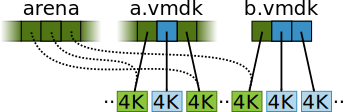
\includegraphics[scale=0.45]{figures/virtualarena.pdf}
  \caption{The virtual arena file appears to contain all shared blocks
    in the file system, but only by way of reference to blocks shared
    by other files.}
  \label{fig:virtual-arena}
\end{figure}
\fi

The virtual arena is a regular file, but unlike typical files, it
doesn't have any data blocks allocated specifically for it (hence, it
is virtual).  Rather, it serves as an alternate view of all shared
blocks in the file
system.  In this way, it is very different from the arenas used in
other deduplication systems such as Venti~\cite{quinlan02venti}, which
store actual data blocks addressed by content addresses.

In order to make a block shared, a host introduces an additional COW
reference to that block from the virtual arena file, using the same
interface that allows blocks to be shared between any two
files.  Apart from uncollected garbage blocks, the virtual arena
consumes only the space of its inode and any necessary pointer
blocks.  Furthermore, this approach takes advantage of the file
system's block placement policies: adding a block to the virtual arena
does \emph{not} move
it on disk, so it is likely to remain sequential with the original
file.

The index can then refer to any shared block by its \emph{offset} in
the virtual arena file, which the file system can internally resolve
to a block address, just as it would for any other file.  The virtual
arena file's inode and pointer block structure exactly form the
necessary map from the abstract, stable block identifiers required by
the index to the block addresses required by the file system.

\subsubsection{On-disk Index Representation}
\label{sec:index:representation}

\DeDe stores the index on disk as a packed list of entries,
sorted by hash.  Because \DeDe always updates the index in large
batches and since the hashes of updates exhibit no spatial
locality, our update process simply scans the entire index file
linearly in tandem with a sorted list of updates, merging the two lists
to produce a new index file.  Despite the simplicity of this
approach, it outperforms common index structures optimized for
individual random accesses (\eg, hash tables and B-trees) even if the
update batch size is small.  Given an average index
entry size of $b$ bytes, a sequential IO rate of $s$ bytes per second,
and an average seek time of $k$ seconds, the time required to apply
$U$ updates using random access is $Uk$, whereas the time to
scan and rewrite
an index of $I$ entries sequentially is $\nicefrac{2Ib}{s}$.  If the
ratio of the batch size to the index size exceeds
$\nicefrac{U}{I} = \nicefrac{2b}{sk}$, sequentially rewriting the
entire index is faster than applying each update individually.
For example, given an entry size of $23$
bytes and assuming a respectable SAN array capable of 150~MB/s and
8~ms seeks, the batch size only needs to exceed $0.004\%$ of the index
size.  Furthermore, hosts defer index updates until the batch size
exceeds some fixed fraction of the index size (at least $0.004\%$), so
the amortized update cost remains
constant regardless of index size.

% b = record size in bytes
% s = sequential IO rate in bytes per second
% k = average seek time in seconds
% |I| = index size in bytes
% n = number of update in a batch

% Where is the inflection point?
% * seconds for sequential update = 2*|I|/s
% * seconds for random update = nk
% * at the inflection point, 2*|I|/s = nk
% * rearrange to get
%   nb/|I| = the ratio of update size to index size
%          = 2b/sk

% RAID'd SAN
% (let* ((K 1024) (b 23) (s (* 150 K K)) (k 8e-3)) (* 100 (/ (* 2 b) (* s k))))

% Average, good disk
% (let* ((K 1024) (b 23) (s (* 70 K K)) (k 8e-3)) (* 100 (/ (* 2 b) (* s k))))

% Worst case
% (let* ((K 1024) (b 23) (s (* 50 K K)) (k 5e-3)) (* 100 (/ (* 2 b) (* s k))))

In order to allow access to the index to scale with the number of
hosts sharing the file system, while still relying on file locking to
prevent conflicting index access, hosts {\it shard} the index into multiple
files, each representing some subdivision of the hash space.  Once the
time a host takes to update a shard exceeds some threshold, the next
host to update that shard will split the hash range covered by the
shard in
half and write out the two resulting sub-shards in separate files.  This
technique mirrors that of extensible
hashing~\cite{fagin79extendiblehashing}, but instead of bounding the
size of hash buckets, we bound the time required to update them.
Combined with file locking, this dynamically adjusts the concurrency
of the index to match demand.

\subsection{Indexing and Duplicate Elimination}

As the index update process incorporates information about recently
modified blocks recorded in the write logs, in addition to detecting
hash matches that indicate potential duplicates, it also performs
the actual COW sharing operations to eliminate these duplicates.  The
duplicate elimination process must be interleaved with the index
scanning process because the results of block content verification can
affect the resulting index entries.
% We begin with an explanation of this process
% assuming only a single host, then describe the changes necessary to
% support multiple hosts, and finally discuss garbage collection.

In order to update the index, a host sorts the recent write
records by hash and traverses this sorted list of write records in
tandem with the sorted entries in the index.  A matching hash between
the two indicates a potential duplicate, which is handled differently
depending on the state of the matching index entry.
Figure~\ref{fig:index-states} gives an overview of all possible
transitions a matching index entry can undergo, given it current
state.

\captionsetup[subfloat]{subrefformat=parens}

\begin{figure}
  \centering
  %
  \subfloat[When the hash $H$ of the block at offset $o$ in file $f$
  is not in the index, a new unique entry is added.]
           {\label{fig:new-unique}
             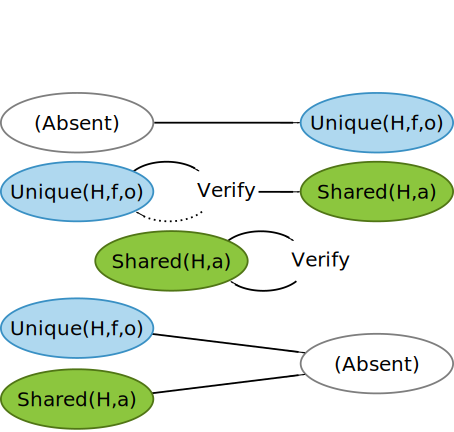
\includegraphics[scale=0.45,viewport=0 220 364
               275,clip]{figures/indexstates.pdf}} \\
%
  \subfloat[When a second occurrence of hash $H$ is found and the
    block's content passes verification, we place it in the virtual
    arena and upgrade the index entry to shared.]
           {\label{fig:unique-to-shared}
             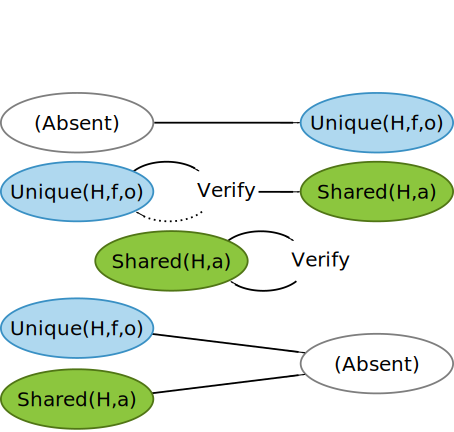
\includegraphics[scale=0.45,viewport=0 165 364
               220,clip]{figures/indexstates.pdf}} \\
%
  \subfloat[When a duplicate of a shared block is found, we
    verify its contents and replace the block with a reference to the
    existing shared block.]
           {\label{fig:shared-to-shared}
             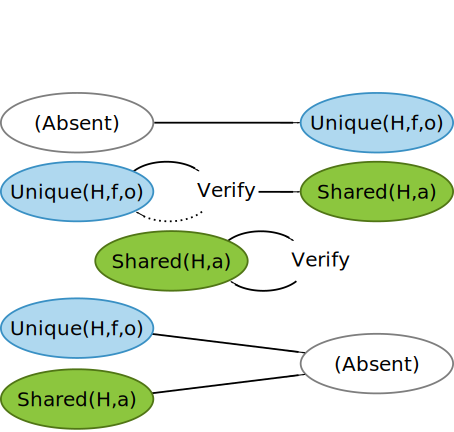
\includegraphics[scale=0.45,viewport=0 110 364
               165,clip]{figures/indexstates.pdf}} \\
%
  \subfloat[Unique entries are garbage collected when the indexing
    process finds a write record to that block with a different hash.
    Shared entries are garbage collected when only the reference from
    the virtual arena remains.]
           {\label{fig:gc}
             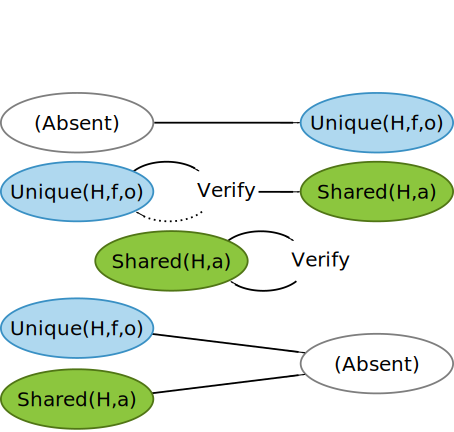
\includegraphics[scale=0.45,viewport=0
               0 364 110,clip]{figures/indexstates.pdf}} \\
%
  \caption{All possible updates to an index entry.}
  \label{fig:index-states}
\end{figure}

When \DeDe detects a potential duplicate, it depends on the file
system's compare-and-share operation, described in
Section~\ref{sec:idea:compare-and-share}, to atomically verify that
the block's content has not changed and replace it with a COW
reference to another block.  Based on user-specified policy, this
verification can either be done by reading the contents of the
potential duplicate block and ensuring that it matches the expected
hash (\ie, compare-by-hash), or by reading the contents of \emph{both}
blocks and performing a bit-wise comparison (\ie, compare-by-value).
If the latter policy is in effect, hash collisions reduce \DeDe's
effectiveness, but do \emph{not} affect its correctness.  Furthermore,
because hashes are used solely for finding potential duplicates, if
\shaone is ever broken, \DeDe has the unique capability of gracefully
switching to a different hash function by simply rebuilding its index.
The content verification step can be skipped altogether if a host can
prove that a block has not changed; for example, if it has held the
lock on the file containing the block for the entire duration since
the write record was generated and no write records have been dropped.
While this is a fairly specific condition, it is often met in \DeDe's
target setting because locks on VM disks are usually held for very
long durations.

\subsubsection{Single Host Indexing}

We begin with an explanation of the index update process assuming only
a single host with exclusive access to the file system.  In a single
host design, the host can modify the metadata of any file.  We lift
this assumption in the next section, where we extend the process to
support multiple hosts.

Any write record without a corresponding hash in the index indicates a
new, unique block.  Even though this write record may be stale,
because index entries for unique blocks are only hints, it is
safe to simply add the new unique block to the index without verifying
the block's content, performing an \emph{absent-to-unique}
transition as shown in
Figure~\subref*{fig:new-unique}.  This single
sequential, buffered write to the index is the only IO incurred when
processing a new unique block.

When a write record's hash corresponds to an index entry for a
unique block, then the host attempts to share both blocks (freeing one
of them in the process) and upgrade the index entry to refer to the
shared block.  This \emph{unique-to-shared} transition is shown in
Figure~\subref*{fig:unique-to-shared}.  However,
because the write record and index entry may both be stale,
the host must verify the contents of both blocks before actually
sharing them.  Assuming this verification succeeds, the file system
replaces both blocks with a shared block and the host inserts
this block into the virtual arena and upgrades the index entry to
refer to the new, shared block.

Finally, if a write record's hash matches an index entry for a
shared block, then the host attempts to eliminate this newly detected
potential duplicate, performing a \emph{shared-to-shared} transition
as shown in
Figure~\subref*{fig:shared-to-shared}.  Because
the write record may be stale, it first verifies that the content of
the potential duplicate has not changed.  If this succeeds, then this
block is freed and the reference to the block is replaced with a
reference to the shared block found via the virtual arena.

\subsubsection{Multi-Host Indexing}

Extending the index update process to multiple hosts, we can no longer
assume that a host will have unfettered access to every file.  In
particular, hosts can only verify blocks and modify block pointers in
files they hold exclusive locks on.  As a result, indexing \emph{must}
be distributed across hosts.  At the same time, we must minimize
communication between hosts, given the cost of communicating via the
shared disk.  Thus, sharing of blocks is done without
any blocking communication between hosts, even if the blocks involved
are in use by different hosts.

In the multi-host setting, the write logs are divided amongst the
hosts according to which files each host has (or can gain) exclusive
access to.  While this is necessary because hosts can only process
write records from files they hold exclusive locks on, it also serves
to divide the deduplication workload between the hosts.

Absent-to-unique transitions and shared-to-shared transitions are
the same in the multi-host setting as in the single host setting.
Adding a new, unique block to the
index requires neither block verification, nor modifying block
pointers.  Shared-to-shared transitions only verify and rewrite blocks
in the file referenced by the current write log, which the host
processing the write log must have an exclusive lock on.

Unique-to-shared transitions, however, are complicated by the
possibility that the file containing the
unique block referenced by the index may be locked by some host other
than the host processing the write record.  While this host
may not have access to the indexed block, it does
have access to the block referred to by the write log.  The host
verifies this
block's content and promotes it to a shared block by adding it to the
virtual arena and upgrading the index entry accordingly.  However, in
order to reclaim the originally indexed block, the host must
communicate this deduplication opportunity to the host holding the
exclusive lock on the file containing the originally indexed block
using the associated merge request file.  The host updating
the index posts a merge request for the file containing the originally
indexed block.  This request contains not only
the offset of the unique block, but also another COW reference to the
shared block.  Hosts periodically check for merge requests to the files
they have exclusive locks on, verifying any requests they
find and merging blocks that pass verification.  The COW
reference to the shared block in the merge request allows hosts to
process requests without accessing the arena.

% Hosts periodically check the merge logs of
% the files they have exclusive locks on, verifying any merge hints that
% they find and merging blocks that pass verification.  Including a COW
% reference to the shared block in the merge hint allows hosts to
% process merge logs without locking the arena.

\subsubsection{Garbage Collection}

As the host scans the index for hash matches, it also
garbage collects unused shared blocks and stale index entries, as
shown in Figure~\subref*{fig:gc}.  For each 
shared block in the index, it checks the file system's reference count
for that block.  If the block is no longer in use, it will have only a
single reference (from the virtual arena), indicating that it can be removed
from the virtual arena and freed.  In effect, this implements a simple form of
weak references without modifying file system semantics.  Furthermore,
this approach allows the virtual arena to double as a victim cache before
garbage collection has a chance to remove unused blocks.

Unique blocks do not need to be freed, but they can leave behind stale
index entries.  Hosts garbage collect these by removing any index entries
that refer to any block in any of the write records being processed by
the host.  In the presence of dropped write records, this may not remove
all stale index entries, but it will ensure that there is at most one
index entry per unique block.  In this case, any later write or potential
duplicate discovery involving a block with a stale index entry will
remove or replace the stale entry.  The garbage collection process
also check for file truncations and deletions and removes any
appropriate index entries.




% \subsection{Index Merging}

% Merging is the process by which an index is updated to include newly
% written data from write logs. In \DeDe, the merging task must be
% distributed across hosts. We avoid involving multiple hosts
% simultaneously because communications is expensive and introduces
% complex failure modes.  So, sharing of blocks is done without
% interactive involvement of multiple hosts, even if the blocks involved
% are in use by different hosts.

% The pending updates to the index stored in the write logs are divided
% amongst the hosts according to which files each host has exclusive
% access to.  While this is necessary because hosts can only process
% updates from files they hold exclusive locks on, it also serves to
% divide the deduplication workload between the hosts.  Once a host has
% accumulated enough pending updates, it updates the index, eliminates
% duplicate blocks, and garbage collects the shared block arena in one
% interleaved process.\XXX[mention figure]

% Figure~\ref{fig:indexing-merging} shows the main parts of the system
% before (left) and after a merge operation. Hosts process write logs
% for their files against the index and zip the two together. Let's take
% an example of the entry in the index corresponding to the hash
% c277d6... This entry was added as a unique block from c.vmdk by host A
% at some point in time in the past. As part of the depicted merge, the
% write log for a.vmdk from host B also had the same block. So, host B
% converted it from a unique entry (U) to a shared one (S) and added it
% to some unoccupied offset in the arena and stored that offset in
% index entry. As part of that operation, c.vmdk couldn't be updated because
% it was still locked by host B. Therefore host A left a merge request
% for host B in a merge request file. Later on, host B picked up the
% merge request and after verification backed reclaimed its duplicate
% block by changing its file pointer to the same as in the virtual
% arena.

% \XXX[ For shared blocks (S), the
% offset is in the virtual arena file whereas for unique blocks (U), it
% is in a reguar file.]

% The linear index representation affords a simple update process: the
% host sorts the updates by hash and traverses the sorted updates in
% tandem with the sorted on-disk index, zipping the two structures
% together to produce the updated index.
% % For a given updated block, there are three possibilities: the
% % block's hash may simply be missing from the index, it may refer to a
% % shared block, or it may refer to a unique block.
% Each update results in either a local merging operation or a
% cross-host merging operation, depending on the presence and type of
% the corresponding index record.

% \XXX[I still feel like this is too hard to wrap one's head around.  We
% need a better overview of index merging to orient the reader before
% giving the details.]

% \subsubsection{Local Merging}

% When an updated block is either a new unique block or another
% duplicate of an already shared block, then the index update can be
% done entirely local to the host performing deduplication.

% If an updated block's hash is missing from the index, then that block
% is a new, unique block.  Even though the update record might be stale,
% unique index records can also be stale, so a host can simply add a new
% unique record for the block to the index without verifying the block's
% hash.  This single sequential, buffered write to the index is the only
% IO incurred by a unique block update.

% If the updated block's hash corresponds to a shared block in the
% index, then an existing, copy-on-write version of the block is already
% available in the arena.  The host verifies that the block's contents
% haven't changed since the update record (comparing either by hash or
% by value) and merges the block from the arena into the original file
% by overwriting the block pointer in the original file with a copy of
% the block pointer from the arena, freeing the block from the original
% file in the process.

% \subsubsection{Cross-Host Merging}

% The transition from unique to shared is complicated by the possibility
% that the file containing the previously unique block and the file
% containing the newly found duplicate may be locked by different hosts.
% Communications between hosts is expensive because we limit ourselves
% to communicating only through shared files on disk, and any
% synchronous communication would introduce complex failure modes.
% Instead, we avoid entirely the simultaneous involvement of multiple
% hosts through asynchronous \emph{merge hints}.  Much like write log
% files, each regular file may have a corresponding merge log containing
% hints of potential deduplication opportunities suggested by other
% hosts.

% When an updated block's hash corresponds to a unique block in the
% index, the block's contents are no longer unique and the block must be
% shared.  While the host creating the shared block may not have access
% to the unique block referenced by the index, it does have access to
% the newly discovered duplicate block.  It makes this block shared by
% verifying its hash, making a COW reference to the block from a freshly
% allocated slot in the arena, and updating the index to replace the
% unique record with a shared record.  It then initiates a cross-host
% merge by posting a merge hint containing the address of the unique
% block that was referenced by the index as well as a COW reference to
% the newly shared block.  Hosts periodically check the merge logs of
% the files they have exclusive locks on, verifying any merge hints that
% they find and merging blocks that pass verification.  Including a COW
% reference to the shared block in the merge hint allows hosts to
% process merge logs without locking the arena. Our hinting scheme is
% similar to memory deduplication hints in~\cite{waldspurger-osdi}.


% \subsection{Mixed VMFS Block Sizes}
% \label{sec:mixed-block-sizes}
% %%%%%%%%%%%%%%%%%%%%%%%
% %%%% Figure %%%%%%%%%%%
% %%%%%%%%%%%%%%%%%%%%%%%
% 
% \begin{figure}[t]
% (a)
% \centerline {
% 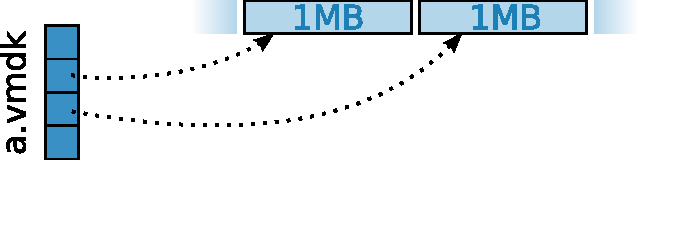
\includegraphics[width=60mm]{figures/1MBsize.pdf}
% }
% (b)
% \centerline {
% 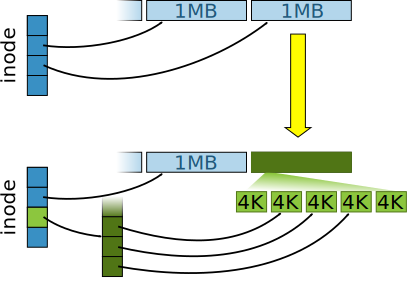
\includegraphics[width=60mm]{figures/mixed.pdf}
% }
% %\vspace{-0.2in}
% \caption{Mixed Block Sizes}
% %\vspace{-0.1in}
% \label{fig:mixed-block-sizes}
% \end{figure}
% 
% %%%%%%%%%%%%%%%%%%%%%%%
% %%%% /Figure %%%%%%%%%%
% %%%%%%%%%%%%%%%%%%%%%%%
% 
% VMFS's 1~MB block allocation unit size minimizes metadata which is ideal
% for allocating large virtual disk files. However, our data suggests
% that deduplication gains diminish with increasing block size. Since
% \DeDe performs deduplication by using file system block pointers,
% large blocks would greatly hinder deduplication. Simply lowering
% the VMFS block size all the way down to 4~KB isn't acceptable since it
% would result in a huge explosion of metadata and go against our design
% goal of introducing no new overhead for unique blocks. Furthermore, small block
% sizes (without additional levels of pointer-block indirection) will not be able
% to address very large files.
% 
% Instead, we added an additional pointer block level of indirection
% which allows individual 1~MB file blocks to be broken into 4~KB blocks,
% shown in Figure~\ref{fig:mixed-block-sizes}.  Note that this is
% different from classical Unix inode structure, which has a fixed
% number of pointer blocks at fixed offsets. We extended VMFS so it can
% dynamically break any 1~MB file block into a pointer block to 256 4~KB
% blocks, based on the specific deduplication requirement, and leave the
% address resolution of other data intact and simple.

\internal{
\subsection{Reducing Temporary File System Bloat}
\label{sec:bloat}

Because \DeDe operates out-of-band, there is a delay between when
duplicate data is written and when \DeDe detects and reclaims this
duplicate data.  This delay allows us to batch updates to the index,
which exposes a trade-off curve between deduplication frequency and
deduplication efficiency (in terms of CPU and IO overhead).  The
approach detailed earlier in this paper optimizes heavily for
efficiency at the cost of frequency; by performing deduplication
only, say, once a day, we can batch up a large number of updates to
the index and drive down the cost of processing each individual
changed block.  Unfortunately, this approach is not always
appropriate.  For example, creating a new virtual machine can
generate a large amount of duplicate data in a very short amount of
time.  Given the delay until deduplication, users may not have
enough additional storage space to withstand such an onslaught of
temporary duplicate data.  We propose two solutions to this problem,
one based on direct knowledge of the source of duplicate data, and
another based on adaptively adjusting the frequency of our
deduplication engine.

First, an examination of the use cases of virtual disks
suggests that new files are often entirely duplicates of some
template virtual disk file.  For example, an IT organization
typically has a small number of operating system images that they
maintain which are used to deploy new VMs to users. This suggests
that we can take care of a significant portion of new data
allocation by supporting an intelligent file clone operation which
instead of performing a {\tt \small cp} would materialized a new
destination file by doing only metadata operations. Since VMFS
already supports COW which \DeDe builds on top of, this is a
relatively simple optimization.

Second, there are reported use cases of users wanting to install
OSes from scratch frequently rather than cloning from templates.
Although we don't yet have any data on how common this scenario is,
we can extend the deduplication engine to support such use cases.
By extending the design of the index, \DeDe can be dramatically more
dynamic, allowing users to control the trade-off between
deduplication frequency and efficiency on a per-file, per-host, or
per-cluster basis.  The index in the current design is a sorted,
completely sequential file that allows extremely efficient batch
updates, but is extremely inefficient at small updates.  Instead, we
can replace this with a variant of a B$^+$-tree (detailed in the
notes below) that supports both efficient batch updates as well as
efficient random updates.  When performing deduplication, the system
can then automatically choose the fastest way to update the index;
either sequentially (which is likely when deduplication is
infrequent such as on the order of days) or randomly (which is
likely when deduplication is frequent such as on the order of
seconds).  Thus, this approach would give users the ability to
dynamically adjust deduplication to their needs and would provide
the option of frequent deduplication when space savings are more
important than peak IO performance.

\begin{itemize}
\item{Jinyuan had an an idea of similarity classes between
  hashes. Something about if some hashes match, you can cache
  index entries of related hashes with high probability of not
  having to visit the index for each one. Thought was it could
  help with things like OS installs where existing images have
  already been seen. Jinyuan needs to fill this in.}
\item Preliminary sketch of the B$^+$-tree index: Divide the index
  into fairly large pages (probably on the order of 64 K, but
  experimentation would be necessary to determine the optimal page
  size).  Each of these pages stores data just like our current
  index does, sorted and delta encoded.  They should be stored
  sequentially as much as possible.  On top of this index, keep
  another index called the jump index that stores the first hash of
  each page (sorted by hash).  Note that this index can be stored
  using exactly the same representation as the base index.  If the
  jump index contains more than one page, store a jump index of the
  jump index, and so forth until the top-most jump index contains
  only a single page.  (It might be reasonable to embed this all in
  one file, more like a traditional B$^+$-tree.)

  When performing a sequential update, read the input index in key
  order (note that this may require seeking around the input index
  if it is not entirely sequential) and write the output index in
  completely sequential order.  Note, however, that some free space
  should be left in each output page to support efficient random
  updates.  The exact amount should probably be learned over time
  based on the observed frequency of page splits.  It will probably
  be small.  When performing random updates, the jump indexes should
  be used to locate the page containing the destination hash.  If
  the update does not cause the page to overflow, it should be
  written back in place (probably via a write to the journal,
  followed by a post-commit copy over the page in the index).  If
  the page does overflow, it should be split into equal halves, the
  first of which should be written back over the original page and
  the second of which should be appended to the end of the index,
  and the jump indexes should be updated (which could cause
  recursive splitting).  When updating the index, the system can
  choose whether sequential or random updates should be faster based
  on the number of updates, the index size, and IO metrics learned
  from previous index updates.

  I also considered using an extensible hash table for the index,
  but this would be strictly less flexible because the nature of the
  structure fixes the average page fullness at 75\% (though, in
  turn, it uses slightly less directory state).  Another alternative
  is to only update the main index during sequential updates and to
  keep a small, separate updates index for random updates.  The main
  index would still need a jump directory, and lookups would
  generally require both an IO to lookup in the update index and an
  IO to lookup in the main index, but this approach has the
  potential to reduce the total amount of IO because the
  probability of a cache hit while writing to the small update index
  is much larger.  Unfortunately, it's really darn hard to analyze.
\end{itemize}
}

\internal{
  \subsection{Storage Migration}
  \label{sec:storage-vmotion}

  Data deduplication for network transfers is a well-studied problem
  with available commercial products that reduce end-to-end data
  transfer times by eliminating redundancy in data traffic. In context
  of our proposed solution, we aim to use content signatures already
  produced and maintained by \DeDe to optimize the higher-level
  application of transferring very large virtual disk files. The
  general sketch is that for blocks on a source host which \DeDe has
  already found to be duplicates, \DeDe already tracks authentic
  hashes. We propose that as part of the application-level connection
  negotiation, \DeDe on the source would provide signatures of the
  {\it shared} blocks of the virtual disk to be transferred. Then, the
  destination host can compare these against its index to know which
  blocks it definitely already has. For such blocks, referred to as
  {\it hits}, the destination informs the source to not send these at
  all, thus saving potentially significant amounts of network traffic
  and therefore latency to completion. Of course, {\it misses} still
  need to be transferred in whatever most optimal way can be
  accomplished by lower layers.

  There are further optimizations that can be built on top of
  this. For example, whenever an index is updated, \DeDe can be
  modified to keep a bloom filter of its contents. Then, using the
  mathematical property of bloom filters that they don't have false
  negatives, we can know definitely which blocks a Storage VMotion
  destination host definitely does {\it not} have. This allows a
  source to receive a small bloom filter as the first step in the
  migration negotiation and immediately start transfer of misses while
  the negotiation of hits continue to happen. Overall, this can help
  in lowering the latency of Storage VMotion even further.

  Some thoughts that need more writing:

  \begin{itemize}
    \item{Cooperates well with the VMAS backed datamover by letting
      that code handle the bulk transfer of unique pages.}
    \item{While unique blocks are received on the dest, it can perform
      dedup on the fly. It already might have the index locked.}
    \item{Need to estimate the cost of index interactions for
      determining if the block hash from a source is available on the
      dest. Should be a single parallelizable index traversal.}
    \item{Investigate using index summary structures to optimize
      lookup of block$\rightarrow$hash}
    \item{Should consider putting hash inside res metadata?}
  \end{itemize}

}

\internal{
  \subsection{Integration with Backup}
  \label{sec:backup-integration}

  Dedupliation is very commonly used in backup and archival systems,
  for example~\cite{quinlan02venti,zhu08datadomain}.
%
%This is due to the fact that a regularly scheduled backup doesn't
%have a lot of data incrementally
%
  Since \DeDe already performs block-level deduplication, it would be
  desirable to integrate with a deduplicating backup system.
  \begin{itemize}
    \item{Backup deduplication engines, including VMware's, typically
      perform variable sized chunking. \DeDe uses fixed-size blocks.}
    \item{We can expose our index format to the backup engine.}
    \item{The basic sketch is that the backup dedup'er would use our
      already computed hashes instead of reading in the block and
      recalculating the hash.}
    \item{How would the backup engine know which block is shared or
      unique. Presumably we could tell it explicitly. How would we
      even figure this out? Given just a file block pointer, we don't
      know if the block is dedup shared or just COW for native
      snapshots. Suppose we did figure it out (see below for ideas),
      then for the shared ones, we would have to flag those
      specifically to the backup engine, which would then have to read
      the index to find their hashes.}
    \item{Should we add a bit to the fb pointer to say the the block
      is dedup shared? This will speed up the ``give me the list of
      shared blocks in this file'' operation}.
    \item{Should we add the hash itself to the fb pointer or the res
      meta data?}
    \item{Note: We have to fence index garbage collection during
      backup window.}
  \end{itemize}

  \subsection{Disaster Recovery}
  \label{sec:dr}
  Sent email to Christos.
}

\internal{
  \subsection{Implementation ToDos}
  \label{sec:todo}
  Dynamic resource pools and a O(1) locality-preserving file block fragmentation operation.
  \begin{itemize}
    \item{If we can simply reassign a 1~MB block from the file block
      pool to the fragment pool, then we can fragment a file block
      purely with metadata operations and maintain complete locality
      and sequentiality of those blocks.}
    \item{It might be possible to make the resource pools even more
      like files, allocated out of some single, global resource
      pool. This is already the design to some extent, as the system
      files appear to be allocated out of the file block resource
      pool. Make them act like thinly allocated files that grow when
      they fill up. The disadvantage to this is that deletions may
      cause fragmentation that leads to space that cannot be reclaimed
      for giving to another resource pool. }
  \end{itemize}
}
